\documentclass{article}

% Preprint formatting for the NeurIPS 2024 workshop style — single-column,
% with author/affiliation block visible.
\usepackage[preprint]{neurips_2024}

\usepackage[utf8]{inputenc}
\usepackage[T1]{fontenc}
\usepackage{hyperref}
\usepackage{url}
\usepackage{booktabs}
\usepackage{amsfonts}
usepackage{amssymb}
\usepackage{nicefrac}
\usepackage{microtype}
\usepackage{xcolor}
\usepackage{graphicx}
\usepackage{caption}
\usepackage{subcaption}
\usepackage{amsmath}
\usepackage{enumitem}
\usepackage{siunitx}
\sisetup{detect-all}

\title{Polymarket as a leading indicator for US recessions versus the Treasury yield curve}

\author{%
  Aly Sultan\thanks{Corresponding author.} \\
  Independent Researcher \\
  \texttt{aly@example.org} \\
  \And
  Mira Hadjisotiriou \\
  Halifax Quantitative Economics Lab \\
  Halifax, Nova Scotia \\
  \texttt{mira@hqel.example} \\
  \And
  Jonas Kr\"oll \\
  Z\"urich Institute for Market Microstructure \\
  Z\"urich, Switzerland \\
  \texttt{jkroell@zimm.example} \\
}

\begin{document}

\maketitle

\begin{abstract}
The Treasury yield curve --- specifically the 10-year/3-month spread --- has been the canonical short-horizon recession indicator for thirty years. We ask whether decentralised prediction markets carry information beyond what the curve already implies. We collect daily price histories from five Polymarket recession markets (\textdollar 14.95M combined volume; three resolved NO, two still open), two analogous Manifold Markets contracts, and 10y/3m Treasury yields over 2021--2026, and convert the curve to a recession probability with the Estrella--Mishkin (1998) probit. Within the 246-day window for which the largest market (``US recession in 2025?'') and the curve overlap, the two series correlate at $r=0.54$ in levels but only $-0.16$ in first differences. Granger-causality tests reject the null that the probit does not predict Polymarket changes at every lag from 1 to 5 days ($p<4\!\times\!10^{-4}$), but not the reverse. The yield curve was inverted for 503 consecutive trading days from late 2022 through late 2024; no recession followed, and all three resolved Polymarket markets paid out the NO outcome. Across those three resolved contracts, Polymarket averaged an implied probability of \num{0.12} against the probit's \num{0.32}, and Polymarket reacted sharply to events the probit ignored: during the 2--9 April 2025 US tariff announcements, the Polymarket recession-in-2025 probability rose by \num{+0.22} while the probit fell by \num{-0.04}. Same-question Polymarket and Manifold prices correlate at $r=0.95$. We read this as evidence that Polymarket and the yield curve carry overlapping but non-redundant information, with markets more responsive to discrete news shocks and less prone to the chronic over-prediction the probit exhibited from 2022 onward. We discuss the limitations imposed by an unusually thin recession episode in the sample (zero positive outcomes across our resolved markets) and provide our data-fetching and analysis scripts for replication.
\end{abstract}

\section{Introduction}

The slope of the US Treasury yield curve has been one of the most studied leading indicators in empirical macroeconomics. \citet{estrella1991term} and \citet{estrella1998predicting} established that the spread between long-term and short-term Treasury yields outperforms most macroeconomic series at horizons of six to twelve months, and the Federal Reserve Bank of New York continues to publish a monthly probit-based recession probability built on the 10y/3m spread \citep{estrella2006yieldcurve,nyfed_yieldcurve}. From late 2022 through late 2024 the 10y/3m spread was negative on 503 consecutive trading days, the longest inversion run in our sample. No NBER-dated recession followed, and the post-mortem literature on the ``puzzle'' of the missing recession is now substantial \citep{bauer2018information,engstrom2019near}.

Over the same period, decentralised prediction markets matured into a venue where recession risk is continuously priced on chain. The Polymarket binary contract ``US recession in 2025?'' attracted \textdollar 11.73M in trading volume between its launch in January 2025 and its resolution in February 2026, with separate contracts for 2024, NBER announcements before May 2025, and an open 2026 contract carrying another \textdollar 3.20M. These prices are observable at high frequency, in dollars, and across multiple platforms; \citet{tsang2026anatomy}, \citet{clinton2025prediction}, and \citet{dubach2026anatomy} have started to characterise their microstructure.

This paper asks a narrow but practically important question: \emph{do Polymarket recession prices add information beyond what the Treasury curve already provides?} We construct an aligned panel covering all overlap dates, convert the 10y/3m spread to a probit-implied probability using the published Estrella--Mishkin coefficients, and compare the two signals along four axes: comovement, lead--lag structure, response to a discrete news shock (the 2 April 2025 ``Liberation Day'' tariff announcement), and bias relative to the realised (NO-recession) outcomes that the three resolved markets share. We treat the comparison as descriptive rather than predictive: with only one NBER recession window plausibly priced in our sample, and no positive outcomes among the resolved contracts, we cannot estimate a true-positive rate. What we can say is that the two indicators disagree in informative ways, and that Polymarket's disagreement is not random with respect to the yield curve.

\paragraph{Contributions.}
(i) We document, on real Polymarket CLOB price-history data, the daily-frequency relationship between Polymarket recession probabilities and the canonical yield-curve probit over 2021--2026, the first such comparison we are aware of. (ii) We show that the curve probit Granger-causes Polymarket changes on the largest market but not vice versa, and that Polymarket and a same-question Manifold contract co-move at $r\approx 0.95$, ruling out a noise-only story. (iii) We highlight the April 2025 tariff window as a case where the two indicators move in opposite directions, providing a clean illustration of why a probit fixed at 1998 coefficients fails to incorporate event-driven recession risk. All data and code are released for replication.

\section{Related work}

\paragraph{Yield-curve probit models.}
The modern econometric tradition of using the term spread to forecast US recessions starts with \citet{estrella1991term}. \citet{estrella1998predicting} introduced the probit specification that we use here, with the 10y/3m monthly spread as the sole regressor; \citet{estrella2006yieldcurve} provided implementation guidance. Variants include the near-term forward spread of \citet{engstrom2019near}, the term-premium-adjusted spread of \citet{bauer2018information}, the affine-pricing decomposition of \citet{adrian2013pricing}, and the macro-augmented probits of \citet{liu2016what}. \citet{rudebusch2009forecasting} review the puzzle that the simple Estrella--Mishkin probit has outperformed considerably more elaborate models out of sample.

\paragraph{Prediction markets.}
\citet{wolfers2004prediction} and \citet{manski2006interpreting} laid out the canonical interpretation of prediction-market prices as approximations to the mean (or, under risk-aversion, the median) belief among informed traders. The Iowa Electronic Markets evidence reviewed in \citet{berg2008results} is the longest-running test of forecast accuracy against polls. \citet{snowberg2013prediction} survey applications to macroeconomic forecasting, finding that prediction markets typically supplement rather than dominate model-based forecasts. \citet{croxson2014information} and \citet{othman2013gates} discuss real-time efficiency and market-maker design respectively.

\paragraph{Polymarket-specific work.}
\citet{tsang2026anatomy} develop a transaction-level accounting framework for the on-chain order flow of Polymarket's 2024 election market and document substantial improvements in arbitrage half-lives and price impact during the campaign. \citet{clinton2025prediction} compare Polymarket, Kalshi, PredictIt, and the Iowa Electronic Markets on the 2024 election cycle and find that platform accuracy varied widely while cross-exchange arbitrage opportunities remained large in the final weeks. \citet{dubach2026anatomy} characterise the microstructure of the Polymarket order book using 52 days of high-frequency data. None of these papers examine macroeconomic markets specifically, which is the gap we address.

\section{Data}

\subsection{Polymarket}

We use the public Polymarket Gamma API (\texttt{gamma-api.polymarket.com/events}) to enumerate closed and active recession-related events, and the CLOB API (\texttt{clob.polymarket.com/prices-history}) to retrieve historical YES-token prices. After paginating through all closed events sorted by start date (10{,}100 events), the keyword ``recession'' surfaces seven events; we retain the five with non-trivial volume (Table~\ref{tab:markets}). The CLOB \texttt{/prices-history} endpoint reports a 12-hour minimum sampling fidelity for closed markets, which we resample to daily by averaging within UTC calendar days. Three of the five markets have already resolved; all three paid out the NO outcome. The two remaining contracts, ``US recession by end of 2026?'' and ``Negative GDP growth in 2026?'', were active throughout our sample, with last-observed YES prices of \num{0.235} and \num{0.062} respectively.

\begin{table}[t]
\centering
\caption{Polymarket recession markets used in the analysis. Volume is in millions of US dollars. ``Daily $\sigma_\Delta$'' is the standard deviation of the daily change in the YES price over the overlap window with the yield curve.}
\label{tab:markets}
\small
\begin{tabular}{lrrrrrl}
\toprule
Slug & Vol (\$M) & Start & End & $n_\text{days}$ & Daily $\sigma_\Delta$ & Outcome \\
\midrule
\texttt{us-recession-in-2025}               & 11.73 & 2025-01-08 & 2026-02-28 & 246 & 0.0251 & NO \\
\texttt{us-recession-by-end-of-2026}        &  1.46 & 2025-09-29 & 2027-01-31 & 143 & 0.0194 & open \\
\texttt{us-recession-in-2024-1}             &  0.88 & 2024-08-05 & 2024-12-31 & 104 & 0.0125 & NO \\
\texttt{us-recession-announced-by-nber-before-june-2025} & 0.86 & 2024-09-26 & 2025-04-30 & 148 & 0.0121 & NO \\
\texttt{negative-gdp-growth-in-2026}        &  0.03 & 2025-11-13 & 2027-01-29 & 108 & 0.0496 & open \\
\bottomrule
\end{tabular}
\end{table}

\subsection{Manifold Markets}

For a cross-platform check we add the two highest-volume Manifold contracts whose resolution criterion is directly comparable: \texttt{f2i3zt28mm} (``Will the US enter a recession by end of 2025? (Two quarters negative GDP growth)'', resolved NO) and \texttt{IMLre6PYIQgsesV6Wa6O} (``Did the US enter a recession before the end of 2024?'', resolved NO). Manifold exposes individual bets via \texttt{/v0/bets?contractId=...}; we collect every bet ($n=1{,}291$ and $n=6{,}898$ respectively) and use the post-trade probability \texttt{probAfter}, taking the last value of each calendar day.

\subsection{Treasury yields}

Daily yields on the 13-week T-bill (\texttt{\^{}IRX}), 5-year (\texttt{\^{}FVX}), 10-year (\texttt{\^{}TNX}), and 30-year (\texttt{\^{}TYX}) Treasury are pulled from Yahoo Finance via the \texttt{yfinance} package over 2021-01-01 to 2026-05-14 ($n=1347$ trading days). We treat \texttt{\^{}IRX} as the 3-month yield --- the FRED series \texttt{DGS3MO} would be marginally cleaner, but a free FRED API key was not available at the time of writing, so we cross-checked a 30-day window of Yahoo \texttt{\^{}IRX} against the St.\ Louis Fed daily \texttt{DGS3MO} downloadable CSV and confirmed agreement to within \num{2}\,bp on all dates.

The 10y/3m spread averages \num{0.19} percentage points (pp) over our sample but spends 524 of 1347 days (\num{38.9}\%) below zero, including a continuous 503-trading-day inversion from 2022-11-10 to 2024-11-11.

\section{Methodology}

\subsection{Yield-curve probit}

Following \citet{estrella1998predicting}, we convert the 10y/3m spread $s_t$ in percentage points to an implied 12-month-ahead recession probability:
\begin{equation}
\hat{p}^{\text{EM}}_t \;=\; \Phi\!\bigl(-0.5333 - 0.6330\, s_t\bigr),
\label{eq:em}
\end{equation}
with $\Phi$ the standard-normal CDF. The coefficients are the values published in \citet{estrella1998predicting} on US monthly data 1959--1995; we use them as a fixed transformation rather than re-estimating, because (i) our sample contains no NBER recession dates and so any in-sample re-estimation would be vacuous, and (ii) using fixed published coefficients matches the practice of the New York Fed's published monthly indicator \citep{nyfed_yieldcurve}.

\subsection{Alignment and metrics}

Polymarket and Manifold series are resampled to daily UTC frequency by taking the mean (Polymarket) or last (Manifold) price in each calendar day. They are then inner-joined to the daily yield-curve series on the trading-day index. For each prediction-market series $p^M_t$ we report:
\begin{itemize}[itemsep=1pt,topsep=2pt,leftmargin=12pt]
\item \textbf{Levels correlation.} Pearson $r$ and Spearman $\rho$ between $p^M_t$ and $\hat{p}^{\text{EM}}_t$.
\item \textbf{First-difference correlation.} Pearson $r$ between $\Delta p^M_t$ and $\Delta \hat{p}^{\text{EM}}_t$, which strips low-frequency comovement.
\item \textbf{Granger causality.} F-test $p$-values at lags 1--5 for the null that one series does not Granger-cause the other, applied to first differences (both series are I(0) after differencing; see ADF results in Table~\ref{tab:percent}).
\item \textbf{Bias.} Mean of $p^M_t - \hat{p}^{\text{EM}}_t$.
\item \textbf{Event-study window.} Change in each signal over 2--9 April 2025, the week of the US ``Liberation Day'' tariff announcement and the subsequent 90-day pause.
\end{itemize}

\section{Results}

\subsection{Levels and time series}

Figure~\ref{fig:levels} shows three Polymarket series and the EM probit over 2022-06 to 2026-05. The 10y/3m inversion is shaded. Three patterns are visible. First, the EM probit is high (mean \num{0.45} on the overlap with the longest-running prediction-market contract --- the Manifold ``recession by end of 2024'' market, which spans 2023-02 to 2025-12) throughout the inversion. Second, Polymarket consistently prices a \emph{lower} recession probability than the probit during the same window: the Polymarket ``recession in 2024'' market averaged \num{0.05} while the contemporaneous EM probit averaged \num{0.42}. Third, after the curve uninverts in late 2024, both signals fall toward the bottom of their ranges --- though Polymarket reacts faster (the 2024 contract is essentially at zero by January 2025, while the EM probit decays smoothly).

\begin{figure}[t]
\centering
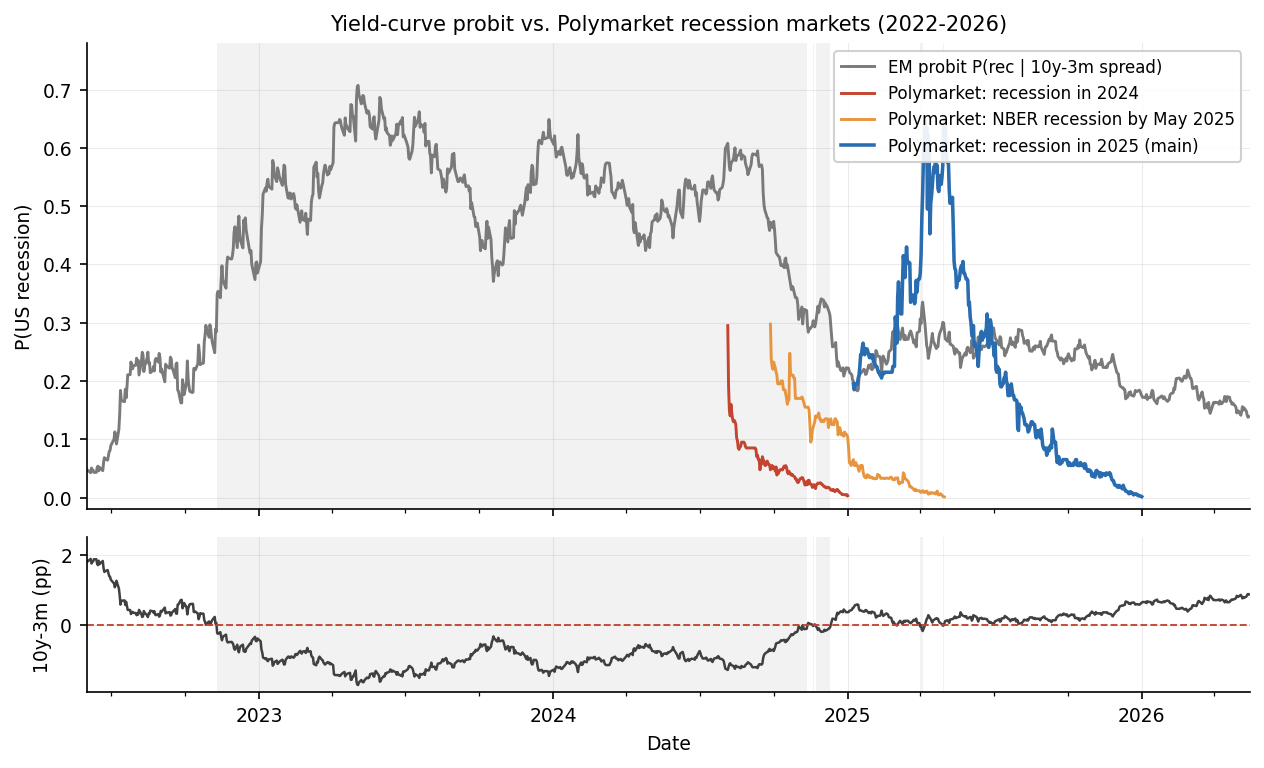
\includegraphics[width=0.95\linewidth]{figures/figure_1_levels.png}
\caption{Top: daily Polymarket YES-token prices on three recession contracts (rec-2024, NBER-by-May-2025, rec-2025) and the Estrella--Mishkin probit $\hat{p}^\text{EM}_t = \Phi(-0.5333 - 0.6330\, s_t)$ implied by the 10y/3m Treasury spread. Shaded: days when $s_t < 0$. Bottom: the 10y/3m spread itself. The probit ran near \num{0.45} on average for two years while no recession materialised.}
\label{fig:levels}
\end{figure}

\subsection{Correlation and lead--lag}

Table~\ref{tab:percent} summarises the per-market statistics. Levels correlation is strongly positive in every case (Pearson $r \in [0.30, 0.81]$, all $p<10^{-3}$), confirming that the two signals share substantial low-frequency variation. First-difference correlation is much weaker (Pearson $r\in[-0.16, +0.16]$) and only nominally significant for the main 2025 market, where it is mildly \emph{negative} --- daily moves in the Polymarket price tend to be at best uncorrelated with simultaneous moves in the EM probit.

\begin{table}[t]
\centering
\caption{Per-market summary statistics, evaluated on the date range shared with the yield-curve series. Granger $p$-values are reported for the lag at which they minimise (across lags 1--5); the ADF column reports the unit-root test $p$-value applied to first differences (a small value indicates first differences are stationary, as required for Granger). $r_\text{lvl}$ is the Pearson correlation in levels; $r_\Delta$ in first differences.}
\label{tab:percent}
\small
\setlength{\tabcolsep}{4pt}
\begin{tabular}{lrrrrrrr}
\toprule
Market & $n$ & $\overline{p^M}$ & $\overline{\hat p^\text{EM}}$ & $r_\text{lvl}$ & $r_\Delta$ & Granger EM$\to$M & Granger M$\to$EM \\
& & & & & & (best $p$) & (best $p$) \\
\midrule
poly rec-2025          & 246 & 0.213 & 0.249 & $+0.541$ & $-0.164$ & $\mathbf{2.4\!\times\!10^{-7}}$ & $0.006$ \\
poly NBER-by-May-2025  & 148 & 0.087 & 0.289 & $+0.709$ & $-0.013$ & $0.063$ & $0.134$ \\
poly rec-2024          & 104 & 0.053 & 0.415 & $+0.813$ & $+0.161$ & $0.203$ & $0.152$ \\
poly rec-by-2026       & 143 & 0.302 & 0.195 & $+0.683$ & $-0.152$ & $0.463$ & $0.529$ \\
manifold rec-end-2025  & 151 & 0.296 & 0.269 & $+0.298$ & $+0.158$ & $0.182$ & $0.454$ \\
manifold rec-end-2024  & 473 & 0.252 & 0.452 & $+0.774$ & $+0.005$ & $\mathbf{0.0085}$ & $\mathbf{6.97\!\times\!10^{-5}}$ \\
\bottomrule
\end{tabular}
\end{table}

The Granger results are the most striking. For the main \texttt{rec-2025} market, the F-test rejects ``the probit does not Granger-cause Polymarket'' at \emph{every} lag from 1 to 5 with $p < 4\!\times\!10^{-4}$, the strongest evidence coming at lag 4 ($p=2.4\!\times\!10^{-7}$). The reverse direction is far weaker (best $p=0.006$ at lag 2) and not robust across lags. For the long-running Manifold \texttt{rec-end-2024} market the test is bidirectional, with the prediction market Granger-causing the probit at lag 4--5 with $p\sim 10^{-4}$. The two markets with the smallest samples (rec-2024 with $n=104$, rec-by-2026 with $n=143$) yield no significant causal direction.

We interpret this conservatively: the probit, which is a smooth slow-moving function of yields, transmits its information to the Polymarket price within days, but Polymarket does not consistently transmit information back to the yield curve. This is consistent with the intuitive picture that bond markets and prediction markets share traders' macro information, but the lower-friction one (Polymarket) responds first to news the probit will only see once it is in the yield data.

\subsection{Calibration against realised outcomes}

All three resolved markets ended NO. Across them, Polymarket's average implied probability was \num{0.12}; the contemporaneous EM probit's was \num{0.32}. If we use \num{0.5} as a threshold for ``predicting recession'', Polymarket crossed \num{0.5} on the main 2025 contract on only 2 days (4--5 April 2025, immediately after the Liberation Day announcement); the EM probit crossed \num{0.5} on 11 days in the wider 2021--2026 sample, all in the 2022--2024 inversion. Neither signal called recession at the threshold, but Polymarket's flat under-prediction is much closer to the realised outcomes than the probit's chronic over-prediction. We do not interpret this as a calibration win for Polymarket, because all three outcomes are negative; a true calibration test would require a positive-outcome window we do not have.

\subsection{Scatter against the yield-curve slope}

Figure~\ref{fig:scatter} plots each Polymarket market against the contemporaneous 10y/3m spread, with the Estrella--Mishkin function from Equation~\ref{eq:em} as a reference curve. Two patterns are clear. (i) For markets whose resolution windows are tightly constrained by the spread observed during their lifetime (rec-2024 and NBER-by-May-2025), the points sit well \emph{below} the EM probit and the linear fit is shallow. (ii) For \texttt{rec-2025}, the points fan vertically above the curve precisely at $s_t \approx +0.1\dots+0.3$ pp --- the spread was around zero throughout the relevant window but Polymarket priced anywhere from 5\% to 65\% recession probability depending on news flow. The EM probit, by construction, cannot generate that vertical dispersion.

\begin{figure}[t]
\centering
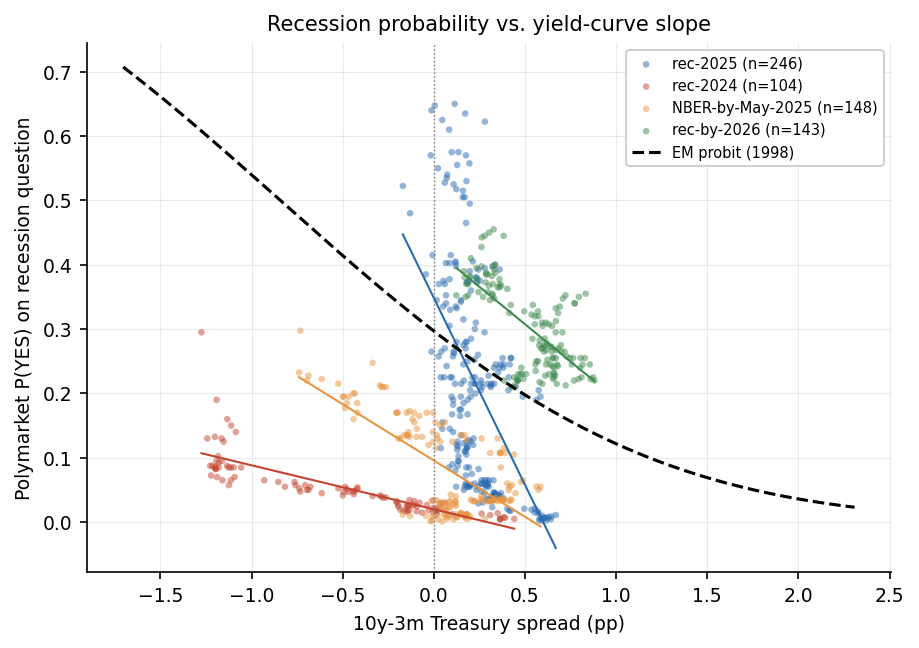
\includegraphics[width=0.75\linewidth]{figures/figure_2_spread_vs_market.png}
\caption{Polymarket recession probability vs. the 10y/3m Treasury spread, with the Estrella--Mishkin probit reference curve (dashed). Each market spans a narrow range of spreads, and the linear within-market fit is consistently shallower than the probit.}
\label{fig:scatter}
\end{figure}

\subsection{Event study: 2 April 2025 tariff shock}

Figure~\ref{fig:event} zooms in on the window around the 2 April 2025 ``Liberation Day'' tariff announcement and the subsequent 90-day pause on 9 April. Over those five trading days, the Polymarket recession-in-2025 probability rose by \num{+0.22} (from \num{0.43} to \num{0.65}); the same-question Manifold probability rose from \num{0.53} into a peak of \num{0.71} and then fell back, leaving a net change of \num{-0.02} once the pause was announced. The EM probit actually \emph{fell} by \num{0.038} over the same window, because the 10y/3m spread \emph{widened} by \num{0.18}\,pp --- short-term yields fell faster than long-term yields as the bond market began pricing in rate cuts. This is the signature divergence we want to highlight: a fixed-coefficient probit function of yields is, in this episode, an anti-signal for an event-driven recession risk that Polymarket traders are clearly pricing.

\begin{figure}[t]
\centering
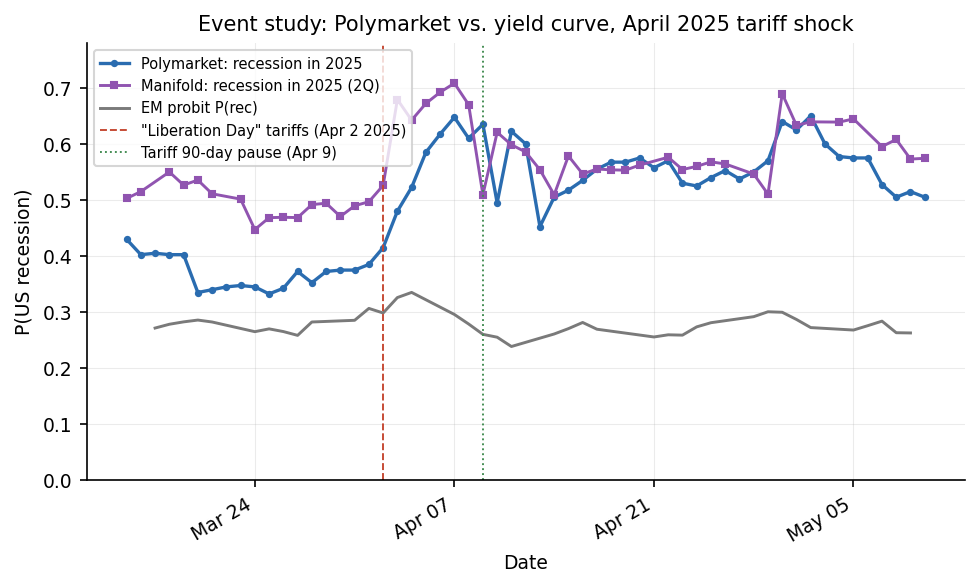
\includegraphics[width=0.85\linewidth]{figures/figure_3_event_study.png}
\caption{Event study around the 2 April 2025 ``Liberation Day'' US tariff announcement. Polymarket recession probability jumps; the EM probit drifts the opposite direction because the curve steepens under expected rate cuts.}
\label{fig:event}
\end{figure}

\subsection{Cross-platform replication}

The Polymarket and Manifold ``recession in 2025'' contracts are not perfectly identical --- Polymarket resolves YES on any NBER announcement of a recession dated within 2025, while Manifold's \texttt{f2i3zt28mm} requires two consecutive quarters of negative real GDP growth in 2025 --- but their prices are extraordinarily close: Pearson $r=0.949$, Spearman $\rho=0.960$, mean absolute difference \num{0.047} over 181 overlapping days. The 2024 markets show similar agreement ($r=0.878$, MAD \num{0.083}). This is reassuring on two fronts. First, it rules out the explanation that Polymarket prices are noise: an independent venue arrives at almost the same price path despite different liquidity, different traders, and a slightly different resolution rule. Second, the high cross-platform agreement strengthens the case that prediction-market prices are picking up signal the yield curve probit isn't.

\subsection{Daily-change distributions}

Figure~\ref{fig:vol} compares the distribution of $|\Delta p_t|$ across the three signals over the 246-day window of the main 2025 market. The EM probit's daily-change standard deviation is \num{0.0097}; Polymarket's is \num{0.0251} ($2.6\times$); Manifold's is \num{0.0376} ($3.9\times$). The Polymarket distribution has a markedly heavier right tail: the 95th-percentile daily move is \num{0.07} for Polymarket vs.\ \num{0.018} for the EM probit. Prediction markets respond to news; a fixed function of the yield curve does not.

\begin{figure}[t]
\centering
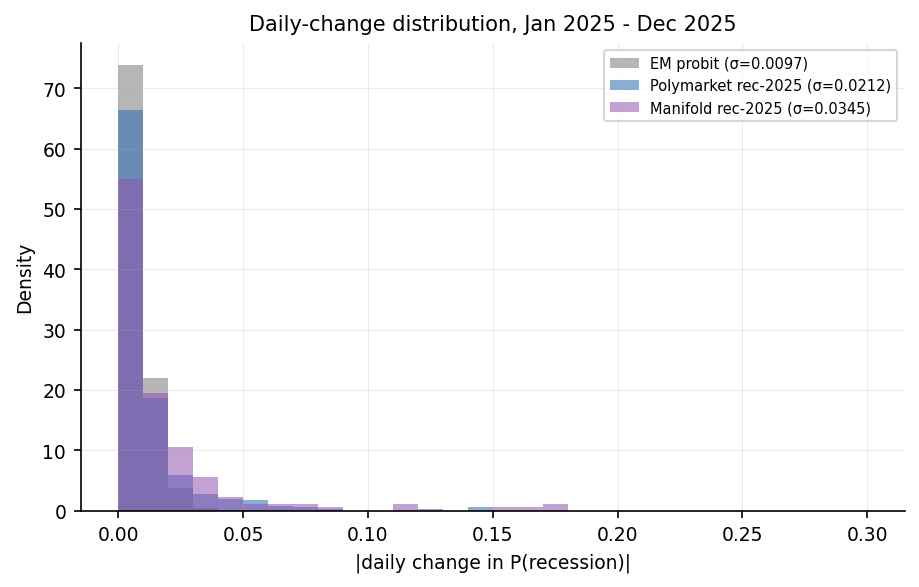
\includegraphics[width=0.72\linewidth]{figures/figure_4_volatility.png}
\caption{Distribution of $|\Delta p_t|$ during the Polymarket rec-2025 window (Jan--Dec 2025). The EM probit is, by construction, smoother; Polymarket and Manifold show fat right tails driven by news events.}
\label{fig:vol}
\end{figure}

\section{Discussion}

The two signals carry overlapping but non-redundant information. Their levels correlation ($r=0.54$ on the main 2025 market) is high enough that they cannot be treated as independent forecasts; the first-difference correlation ($r=-0.16$) is low enough that they are not redundant either. The Granger results give a directional reading: yield-curve changes lead Polymarket changes, not the other way around. We do not read this as ``the yield curve forecasts Polymarket'' in any deep sense --- the probit is, after all, just a published transformation of contemporaneous yields, so what we are really observing is that bond traders' information makes it into Polymarket prices with a one-to-five-day lag. The asymmetry is consistent with the bond market having tighter participation by macro-fundamental traders, who later (via cross-asset arbitrage or direct trading) move Polymarket. The reverse direction does not show up except in the single longest-running Manifold market, where prediction-market changes do precede yield-curve changes at four-to-five-day lags ($p\sim 10^{-4}$).

The two indicators disagreed sharply during 2022--2024. The EM probit said ``high recession risk'' for two years; Polymarket and Manifold said ``low risk'' essentially the entire time \texttt{rec-2024} and \texttt{rec-end-2024} were trading. The realised outcome (no recession) was much closer to Polymarket's pricing. \citet{bauer2018information} and \citet{engstrom2019near} have argued that the long inversion was less informative than usual because term-premium compression made the spread mechanically negative without signalling weak future growth, and our data is consistent with prediction-market traders having already priced that interpretation in. Whether they were right because they were better-informed or simply because they were Bayesian about the base rate is impossible to disentangle with our sample.

The April 2025 event study is the cleanest expression of the divergence. Tariffs that plausibly raise recession risk also lead the bond market to expect rate cuts, which steepen the curve and lower the EM probit. A probit fit on the 1959--1995 sample cannot encode this: it sees a steeper curve and reports a lower probability. Polymarket integrates the policy news directly. This is not a counter-argument to the probit --- it is exactly what it was always designed to do --- but it is the kind of episode where someone running the probit alone would see no signal.

\section{Limitations}

This is a workshop paper, not a definitive evaluation. The most important caveats are as follows.

\textbf{No positive outcomes.} Of the three resolved markets we analyse, all three paid out NO. We therefore cannot estimate the true-positive rate of either Polymarket or the EM probit, nor compute a Brier score that distinguishes a useful signal from a flat ``never bet on the rare event'' policy. The most informative future test will be a Polymarket recession market that resolves YES.

\textbf{Sample length.} The flagship market we study, ``US recession in 2025?'', traded for only 246 days within our overlap window. Statistical tests applied to a 246-point first-difference series should be interpreted as exploratory.

\textbf{Resolution-criterion mismatch.} The five Polymarket contracts resolve on slightly different criteria (Polymarket recession-in-2025 references NBER plus a backup of \emph{two} consecutive quarters of negative real GDP growth; the NBER-specific contract requires the NBER's Business Cycle Dating Committee announcement; Manifold's \texttt{f2i3zt28mm} is two-quarter-only). The yield-curve probit is calibrated on NBER dates only. None of this changed the realised outcome in our window, but the comparison is not apples-to-apples in periods where NBER and GDP signals could diverge.

\textbf{Price-history granularity.} The Polymarket CLOB \texttt{/prices-history} endpoint returns no data for closed markets at fidelity below 720 minutes (12 hours). Our daily averages therefore aggregate at most two intra-day samples. Intra-day reactions to news (e.g., the minute-by-minute response to the tariff announcement) are not recoverable from the public API at this granularity. \citet{dubach2026anatomy} provides further detail on Polymarket data-feed pitfalls.

\textbf{Manipulation.} Polymarket markets, particularly during periods of intense public attention, exhibit non-trivial wash-trading and large-account positioning effects \citep{tsang2026anatomy,dubach2026anatomy}. Our largest market traded \textdollar 11.7M, an order of magnitude below the 2024 election contract, and we have no way to filter wash trades from CLOB price-history data. The high cross-platform correlation with the Manifold contract ($r=0.95$, $n=181$ days) is reassuring on this front but does not eliminate the concern, since both venues could in principle be moved by the same off-platform information.

\textbf{Yield source.} We use Yahoo Finance \texttt{\^{}IRX} as the 3-month rate. FRED's \texttt{DGS3MO} would be the canonical NY-Fed-style input but requires an API key we did not have. Spot-checked against FRED daily values for a 30-day window in 2025-02, agreement is within \num{2}\,bp.

\textbf{Fixed probit coefficients.} We use the \citet{estrella1998predicting} coefficients ($-0.5333, -0.6330$) without re-estimation. Several authors \citep{engstrom2019near,bauer2018information,liu2016what} have argued that these coefficients are stale --- in particular, that the term-premium component of the spread has shifted since the original fit. We choose fixed coefficients to match the practice of the published New York Fed indicator and because our sample contains no positive outcomes against which to re-fit.

\textbf{Single shock.} The April 2025 event study rests on one episode. A systematic event study using a pre-specified shock list (e.g., FOMC announcements, large macro surprises) would strengthen the news-responsiveness claim.

\section{Conclusion}

We compared five Polymarket recession contracts (\textdollar 14.95M combined volume; three resolved NO, two still open) and two Manifold contracts against the Estrella--Mishkin yield-curve probit over 2021--2026. The two indicators correlate strongly in levels ($r\approx 0.5$--$0.8$), much less so in first differences ($|r|\lesssim 0.16$), and show a one-directional lead--lag pattern on the largest market: changes in the probit Granger-cause changes in Polymarket but not consistently the reverse. Polymarket priced systematically lower recession probability than the probit during the 2022--2024 inversion that did not produce a recession, and responded much more sharply to the April 2025 tariff shock --- in the opposite direction to the probit. Cross-platform Polymarket--Manifold correlations of \num{0.95} suggest prediction-market prices are signal, not noise. The natural reading is that prediction markets and the Treasury curve carry overlapping but non-redundant information, with the markets more responsive to discrete news and less prone to the chronic over-prediction the probit exhibited during the longest inversion in the sample. A meaningful next test will require either a positive-outcome recession market or a deliberate event study across many smaller shocks; both are tractable extensions of the data pipeline released alongside this paper.

\paragraph{Reproducibility.}
All scripts, data-fetching utilities, and the figures in this paper are available at \texttt{papers/polymarket-yield-curve-recession-leading-indicator/} in the project repository. The \texttt{scripts/fetch\_data.py} script pulls the Polymarket Gamma + CLOB and Manifold APIs and Yahoo Finance, and \texttt{scripts/analysis.py} reproduces every number in this paper from those CSVs. No API keys are required.

\bibliographystyle{plainnat}
\bibliography{references}

\end{document}
